En esta sección se revisan algunos de los trabajos más importantes en relación a los operadores de cruce.
%
%This section is devoted to review some of the most important works that are highly related to the research presented in this paper.
%
Inicialmente, se definen varios conceptos del campo multi-objetivo.
%First, the most important \MOEAS{} paradigms are defined.
%
Posteriormente, se introducen algunas clasificaciones relevantes de los operadores de cruce.
%Thereafter, some relevant classifications of crossover operators are introduced.
%
Finalmente, es discute el operador de cruce \SBX{} el cual es utilizado de forma extenda en esta sección.
%Finally, the popular \SBX{} operator, which is used extensively in this paper, is discussed.

\subsection{Algoritmos Evolutivos Multi-objetivo}


Un MOP continuo basado en minimización puede ser definido como se indica en la ecuación (\ref{eqn:Model})
%A continuous minimization-based MOP can be defined as indicated in the equation (\ref{eqn:Model}).

\begin{equation}
 \label{eqn:Model}
   \begin{split}
    Minimizar \quad & f_m(\mathbf{x}), \quad m = 1, 2,...,M;\\
   Sujeto \quad a \quad &  x_i^{(L)} \leq x_i \leq x_i^{(U)}, \quad i=1,2,..., n. \\
   & \mathbf{x} \in \Omega
   \end{split}
\end{equation}

donde $\mathbf{n}$ es la dimensión correspondiente al espacio de las variables, $\Omega$ es el espacio factible, $\mathbf{x}$ es un vector compuesto por $\mathbf{n}$ variables de decisión $x=(x_1, ..., x_n) \in R^n$, y $x_i^{(L)}$ y $x_i^{(U)}$ son los límites inferior y superior de cada variable.      


En los últimos años, se han ideado una gran cantidad de \MOEAS{} los cuales siguen distintos principios.
%In the last years, a large number of \MOEAS{} following different design principles have been devised.
%
En orden para mejor tener una mejor clasificacón, se han propuesto varias taxonomías~\cite{Joel:BOOK_MOEAs}.
%In order to better classify them, several taxonomies have been proposed~\cite{Joel:BOOK_MOEAs}.
%
En base a sus principios de diseño, los \MOEAS{} pueden ser basados en la dominancia de Pareto, indicadores y/o descomposición~\cite{pilat2010evolutionary}.
%Attending to the principles of design, \MOEAS{} can be based on Pareto dominance, indicators and/or decomposition~\cite{pilat2010evolutionary}.
%
Todos estos algoritmos son suficientemente competitivos, por lo tanto en esta sección se consideraron \MOEAS{} de distintos grupos.
%All of them have quite competitive representatives, so in this paper \MOEAS{} belonging to the different groups are taken into account.
%
Particularmente, la validación experimental se desarrollo incluyendo a los algoritmos \textit{Algoritmo Genético basado en Ordenación de los No-Dominados} (Non-Dominated Sorting Genetic Algorithm - NSGA-II)~\cite{Joel:NSGAII}, \textit{el MOEA basado en descomposición} (the MOEA based on Decomposition - \MOEAD{})~\cite{Joel:MOEAD} y el \textit{Algoritmo Evolutivo Multi-objetivo basado en la Métrica-S} (the $S$-Metric Selection Evolutionary Multi-objective Optimization Algorithm - \SMSEMOA{})~\cite{Joel:SMSEMOA}.
)
%Particularly, the experimental validation has been carried out by including the Non-Dominated Sorting Genetic Algorithm (NSGA-II)~\cite{Joel:NSGAII}, 
%the MOEA based on Decomposition (\MOEAD{})~\cite{Joel:MOEAD}, and the $S$-Metric Selection Evolutionary Multi-objective Optimization Algorithm (\SMSEMOA{})~\cite{Joel:SMSEMOA}.
%
Estos algoritmos son representantivos de los basados en dominancia, basados en descomposición y basados en indicadores respectivamente.
%They are representative methods of the domination-based, decomposition-based and indicator-based paradigms, respectively.
%
Las siguientes sub-secciones describen cada uno de los paradigmas involucrados en los métodos seleccionados.
%The following subsections briefly describe each one of these paradigms and introduce the selected methods.

\subsubsection{Algoritmos Basados en el concepto de Dominancia - NSGA-II }
%\subsubsection{Domination Based MOEAs - NSGA-II}

Uno de los paradigmas mas reconocidos son los enfoques basados en dominancia.
%One of the most recognized paradigms is the domination based approach.
%
Los \MOEAS{} que pertenecen a esta categoría se basan en la aplicación de la relación de dominancia para diseñar los distintos componentes de los mismos, especialmente en la fase de selección.
%\MOEAS{} belonging to this category are based on the application of the dominance relation to design different components of the EAs, specially the selection phase.
%
Dado que la relación de dominancia no promueve la diversidad de forma implícita en el espacio de los objetivos se han desarrollado técnicas para obtener una diversidad en el espacio de los objetivos como es el niching, crowding y/o clustering que usualmente se integran
%Given that the dominance relation does not inherently promotes diversity in the objective space, auxiliary techniques such as niching, crowding and/or clustering 
%are usually integrated to obtain an acceptable spread and diversity in the objective space.
%
Una debilidad importante en los métodos basados en la relación de dominancia es la escalabilidad en términos de dimensionalidad en el espacio de los objetivos.
%A critical drawback of methods based on the dominance relation is its scalability in terms of the
%dimensionality of the objective space.
%
De hecho la presión de selección es substancialmente reducida conforme el número de objetivos incrementan.
%In fact the selection pressure is substantially reduced as the number of objectives increases.
%
A pesar de que se han desarrollado algunas estrategias para solventar este inconveniente \cite{horoba2008benefits}, este parece ser la debilidad mas importante de este tipo de algoritmos.
%Although some strategies have been developed to deal with this issue \cite{horoba2008benefits} it remains 
%as an important drawback for this kind of algorithms.

El \NSGAII{} es uno de los algoritmos mas importantes de este grupo.
%One of the most popular techniques of this group is the \NSGAII{}.
%
Este algoritmo~\cite{Joel:NSGAII} considera un operador de selección especial el cual está basado en los procedimientos de la ordenación de las soluciones no dominadas y en el amontonamiento.
%This algorithm \cite{Joel:NSGAII} considers a special selection operator
%based on non-dominated sorting and crowding.
%
El procedimiento que realiza la ordenación de las soluciones no dominadas es utiliza para proporcionas convergencia hacia el frente de Pareto mientras que el procedimiento de amontonamiento se utiliza para promover la diversidad en el espacio de los objetivos.
%Non-dominated sorting is used to provide convergence to the Pareto front whereas crowding promotes the preservation of diversity in the objective space.
%
%

%\subsubsection{Decomposition Based MOEAs - MOEA/D}
\subsubsection{Algoritmos multi-objetivo basados en descomposición - MOEA/D}

Los \MOEAS{} basados en descomposición \cite{Joel:MOEAD} transforman un \MOP{} en un conjunto de problemas de optimización mono-objetivo de forma simultánea.
%Decomposition-based \MOEAS{} \cite{Joel:MOEAD} transform a \MOP{} in a set of single-objective optimization problems that are tackled simultaneously.
%
Esta transformación puede ser lograda a través de distintos enfoques.
%This transformation can be achieved through several approaches.
%
Uno de los mas populares es por medio de la función pesada de Tchebycheff la cual requiere un conjunto de pesos bien distribuídos con el propósito de alcanzar soluciones bien distribuídas a lo largo del frente de Pareto.
%The most popular of them is applying a weighted Tchebycheff function, thus requiring a set of well distributed weights to attain well-spread solutions.
%
Sin embargo este tipo de algoritmos poseen una desventaja importante y está relacionada con la geometría que posee el frente de Pareto.
%An important drawback of this kind of approaches is related to the dependency between the Pareto front geometry and the weights required to attain proper solutions.
El \MOEA{}~\cite{Joel:MOEAD} es un \MOEA{} popular de los basados en descomposición.
%\MOEAD{}~\cite{Joel:MOEAD} is a recently designed decomposition-based \MOEA{}.
%
Este incluye varias características, tales como la descomposición de los problemas, la agregación de los pesos con los objetivos y las restricciones de emparejamiento que están basadas en la definición de vecindarios.
%It includes several features such as problem decomposition, weighted aggregation of objectives 
%and mating restrictions based on neighborhood definitions.
%
%Particularly, the neighborhoods are considered in the mating selection.
%
El algoritmo \MOEADDE{} es considerado como una variante popular del \MOEAD{}, el cual utiliza operadores de \DE{}~\cite{price2006differential} y el operador de mutación polinomial~\cite{hamdan2012distribution} en la fase de reemplazo.
%A popular variant of \MOEAD{} is the \MOEADDE{}, which uses the \DE{} operators~\cite{price2006differential} 
%and the polynomial mutation operator~\cite{hamdan2012distribution} in the reproduction phase.
%
Adicionalmente, este algoritmo tiene dos mecanismos especiales para mantener la diversidad de la población~\cite{zhang2009performance}.
%Additionally, it has two extra mechanisms for maintaining the population diversity~\cite{zhang2009performance}.
%

\subsubsection{Algoritmo multi-objetivo basados en indcadores - SMS-EMOA}
%\subsubsection{Indicator Based MOEAs - SMS-EMOA}

En optimización multi-objetivo se han desarrollado varios indicadores de calidad con el propósito de comparar el rendimiento de los \MOEAS{}.
%In multi-objective optimization several quality indicators have been developed to compare the performance of MOEAs.
%
Debido a que estos indicadores miden la calidad de las aproximaciones alcanzadas por los \MOEAS{} se propuso un paradigma basado en en la aplicación de estos indicadores.
%Since these indicators measure the quality of the approximations attained by \MOEAS{}, a paradigm based on the application of these indicators was proposed.
%
Particularmente, los indicadores reemplazan a la relación de dominancia de Pareto con el propósito de guiar el proceso de optimización.
%Particularly, the indicators replace the Pareto dominance relation with the aim of guiding the optimization process.
%
Principalmente, el hypervolúmen es uno de los indicador de calidad ampliamente aceptados denominado por su relación completa de Pareto (Pareto-compliance)~\cite{Joel:IGDPlus_And_GDPlus}.
%Among the different indicators, hypervolume is a widely accepted Pareto-compliance quality indicator~\cite{Joel:IGDPlus_And_GDPlus}.
%
Una de la principales ventajas de estos algoritmos es que los indicadores normalmente consideran tanto la calidad de las soluciones como su diversidad, por lo tanto no se requieren mecanismos adicionales para preservar la diversidad.
%One of the main advantages of these algorithms is that indicators usually take into account both the quality and diversity of the solutions,
%so no additional mechanisms to preserve diversity are required.
%

Un algoritmo popular que utiliza que es basado en indicadores es el \SMSEMOA{}~\cite{Joel:SMSEMOA}.
%A popular and extensively used indicator-based algorithm is the \SMSEMOA{}~\cite{Joel:SMSEMOA}.
%
Este \MOEA{} es considerado como un algoritmo híbrido ya que utiliza tanto indicadores como el concepto de la dominancia de Pareto.
%This algorithm might be considered as hybrid, since it involves both indicators and Pareto dominance concepts.
%
Escencialmente, este algoritmo integra el procedimiento para ordenar a las soluciones no dominadas con la métrica del hipervolúmen.
%Essentially, it integrates the non-dominated sorting method with the use of the hypervolume metric.
%
Por lo tanto el \SMSEMOA{} aplica el hipervolúmen como estimados de densidad siendo una tarea computacionalmente pesado.
%Thus, \SMSEMOA{} uses the hypervolume as a density estimator which results in a computationally expensive task.
%
Particularmente, la fase de reemplazo elimina al individuo que pertenece al frente con peor rango y cuya contribución al hipervolúmen sea mínima.
%Particularly, the replacement phase erases the individual of the worst ranked front with the minimum contribution to the hypervolume.
%
Debido al comportamiento prometedor del \SMSEMOA{} se ha considerado como parte de nuestra validación experimental.
%Taking into account the promising behavior of \SMSEMOA{}, it has been used in our experimental validation.
%

\begin{figure}[!t]
\centering
%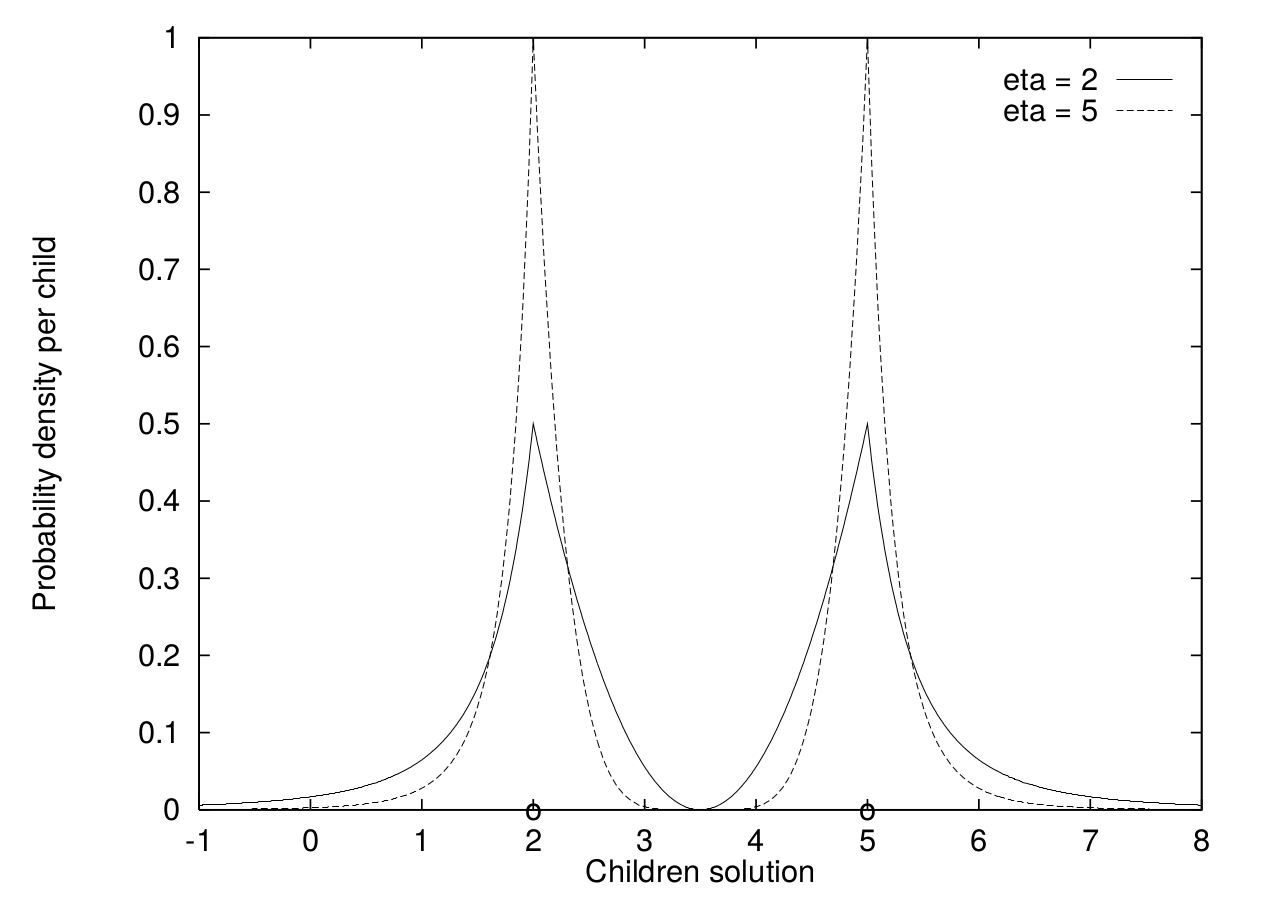
\includegraphics[width=2.5in]{img/Operadores/DensitySBX_English.png}
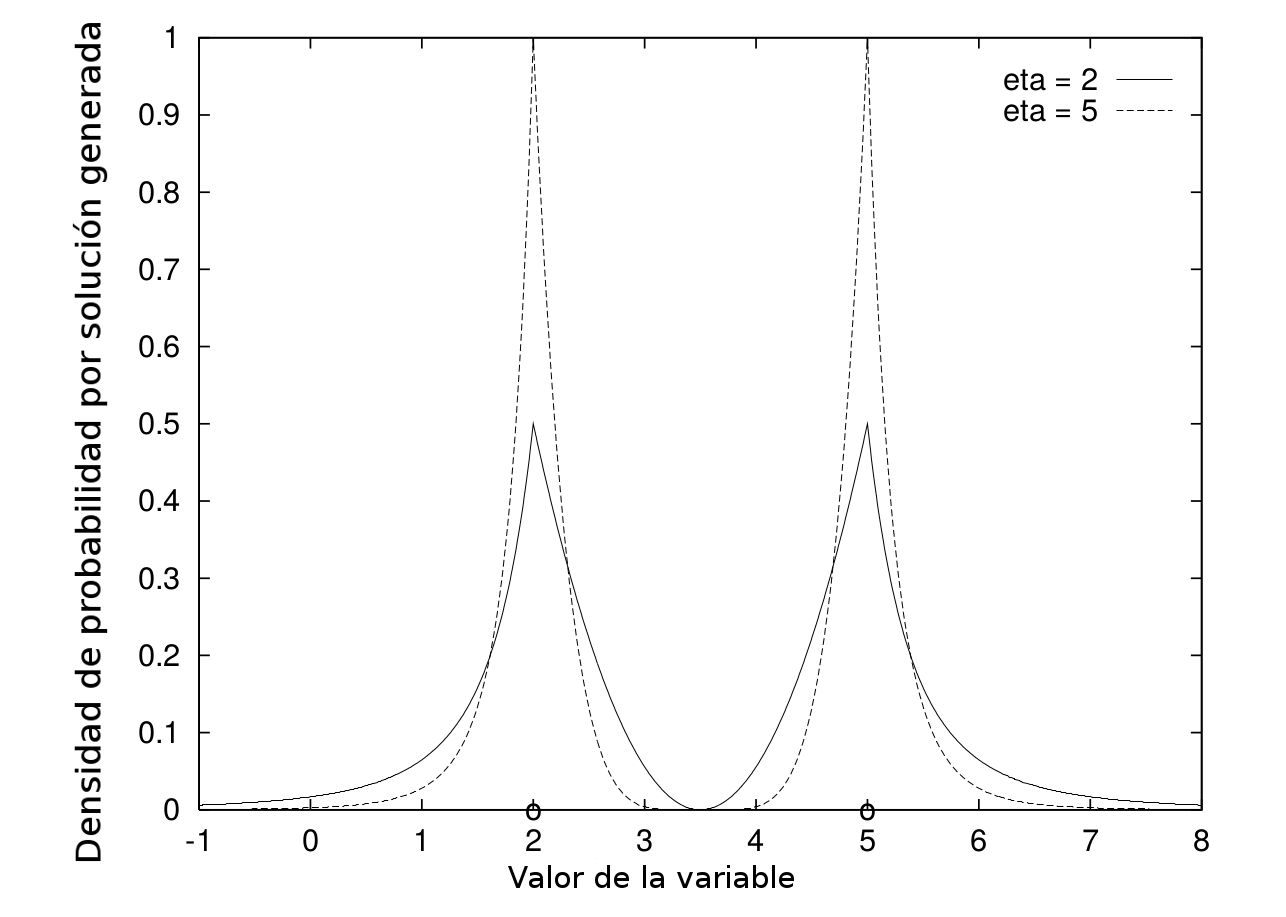
\includegraphics[width=0.5\textwidth]{img/Operadores/DensitySBX.png} 
\caption{Probability density function of the \SBX{} operator with indexes of distribution 2 and 5. The parents are located in 2 and 5 respectively.}
\label{fig:fig_sim}
\end{figure}

\begin{figure}[t]
\centering
\begin{tabular}{cc}
   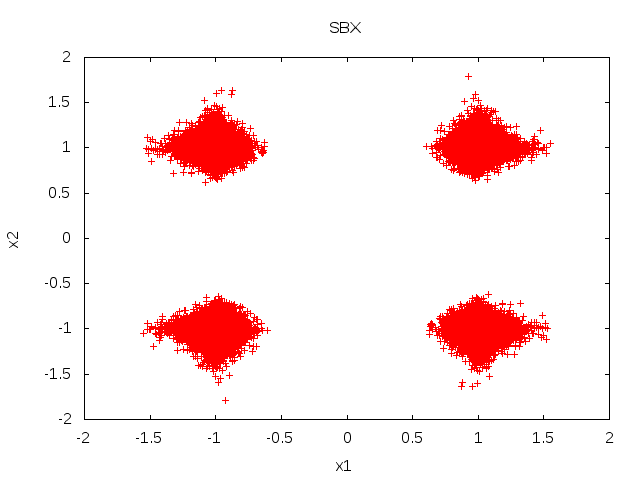
\includegraphics[width=0.23\textwidth]{img/Operadores/SBX_eta_20_2D_pv_1.png} 
   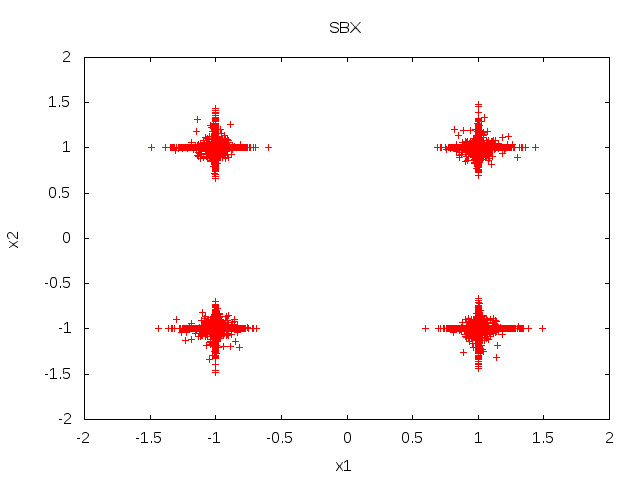
\includegraphics[width=0.23\textwidth]{img/Operadores/SBX_eta_20_2D_pv_01.png} 
\end{tabular}
\caption{Simulations of the \SBX{} operator with a distribution index equal to 20. Parents are located in $P_1=(-1.0, -1.0)$ and $P_2=(1.0, 1.0)$. The left simulation corresponds to a probability of altering a variable ($\delta_1$ in Algorithm \ref{alg:SBX_Operator}) equal to $1.0$ and in the right it corresponds to $0.1$.}
\label{fig:Simulation_pv}
\end{figure}



%
\begin{figure}[t]
\centering
\begin{tabular}{cc}
   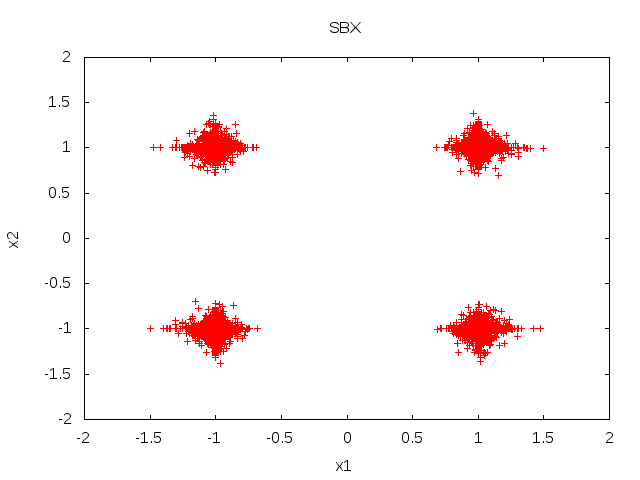
\includegraphics[width=0.23\textwidth]{img/Operadores/SBX_eta_20_2D.png} 
   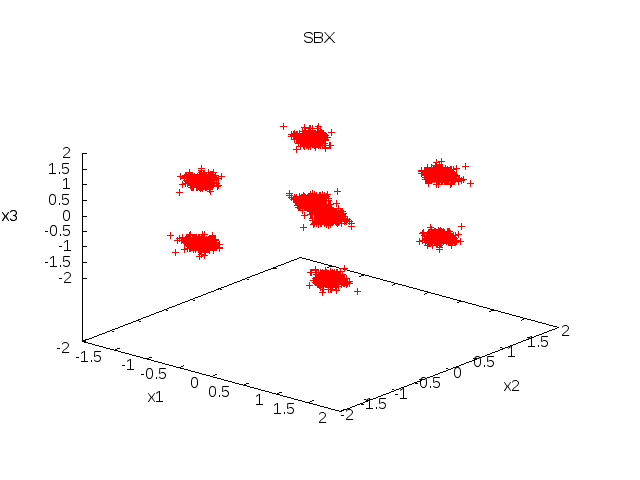
\includegraphics[width=0.23\textwidth]{img/Operadores/SBX_eta_20_3D.png} 
\end{tabular}
\caption{Simulations of the \SBX{} operator with a distribution index equal to 20. Parents are located in $P_1=(-1.0, -1.0)$ and $P_2=(1.0, 1.0)$ and $P_1=(-1.0, -1.0, -1.0)$ and $P_2=(1.0, 1.0, 1.0)$ for two and three variables respectively.}
\label{fig:Simulations_Index_20}
\end{figure}


\subsection{Operadores de cruce}
%\subsection{Crossover operators}

Los operadores de cruce son diseñados para generar soluciones hijo utilizando la información de las soluciones padre.
%The crossover operators are designed to generate offspring solutions using information of the parent solutions.
%
Estos combinan las características de dos o más soluciones padre con el propósito de generar nuevas soluciones candidatas.
%They combine features of two or more parent solutions to generate new candidate solutions.
%
En base a que en la literatura existen varios operadores de cruce se han propuesto varias taxonomías para clasificarlos.
%Since several crossover operators have been proposed, some taxonomies have also been provided.
%
Particularmente, las taxonomías se basan en varias características tales como la ubicación de las nuevas soluciones generadas o por el tipo de relaciones que existen en las variables.
%The taxonomies are based on features such as the location of new generated solutions or the kinds of relations among the variables.

Una taxonomía popular realiza la clasificación de los operadores de cruce en basados en variables o basados en vectores.
%A popular taxonomy classifies crossover operators into variable-wise operators and vector-wise operators.
%
En la categoría donde son basados en las variables, cada variable de las soluciones padre son combinadas para crear nuevos valores, esto se realiza de forma independiente y en base a una probabilidad especificada con anterioridad 
%In the variable wise category, each variable from parent solutions is recombined independently with a certain pre-specified probability to create new values.
%
Este tipo de operadores son ideales para lidiar con problemas separables.
%These operators are specially suitable to deal with separable problems.
%
Algunos operadores que pertenecen a esta categoría son el \textit{Operador de Cruce Ciego} (the Blend Crossover - \BLX{})~\cite{eshelman1993real} y el \SBX~\cite{Joel:SBX1994}.
%Some operators belonging to this category are the Blend Crossover (\BLX{})~\cite{eshelman1993real}, and the \SBX{}~\cite{Joel:SBX1994}.
%
De forma alternativa, los operadores de recombinación basados en vectores son diseñados para considerar la dependencia que existe entre las variables.
%Alternatively, the vector-wise recombination operators are designed to take into account the linkage among variables.
%
Este tipo de operadores regularmente realizan una combinación lineal de las soluciones involucradas.
%They usually perform a linear combination of the variable vectors.
%
Algnos operadores que pertenecen a esta categoría son \textit{El Operador de Cruce Unimodal Normalmente Distribuído} (The Unimodal Normally Distributed Crossover - \UNDX{})~\cite{Joel:UNDX}, y \textit{El Operador de Cruce basado en el Simplex} (The simplex crossover ' \SPX{}) \cite{Joel:DE_Storn_SPX}.
%Some operators belonging to this category are the Unimodal Normally Distributed Crossover (\UNDX{})~\cite{Joel:UNDX}, and the simplex crossover (\SPX{}) \cite{Joel:DE_Storn_SPX}.
%
Adicionalmente, los operadores de cruce pueden ser clasificados como basados en los padres y basados en la media \cite{jain2011parent}.
%Additionally, crossover operators can be classified as Parent-Centric and Mean-Centric \cite{jain2011parent}.
%
En los operadores basados en los padres, las soluciones hijo son creadas alrededor de cada solución padre, mientras que en los operadore basados en la media existen una tendencia de crear a las soluciones hijo alrededor de la media generada por las soluciones padres.
%In Parent-Centric operators, children solutions are created around one of the parent solutions, whereas in Mean-Centric operators, children solutions tend to be created mostly 
%around the mean of the participating parent solutions.
%
Entre los operadores de cruce el \SBX{} es probablemente uno de los más utilizados, por lo tanto esta sección se centra en este operador de cruce.
%Among the crossover operators, \SBX{} is probably the most frequently used operator, so this research focuses on this crossover.

\subsubsection{El Operador de Cruce Basado en Simulación Binaria - SBX}
%\subsubsection{Simulated Binary Crossover - SBX}

Los operadores de reproducción son uno de los componentes mas relevantes para influencias el proceso de búsqueda en los \EAS{}.
%The reproduction operators are one of the most relevant components that influence the search process of \EAS{}.
%
Específicamente, los operadores de cruce y mutación están altamente relacionados con la diversidad de las soluciones.
%Specifically, the crossover and mutation operators are highly related with the diversity of solutions.
%
Por lo tanto, los operadores considerados afectan la calidad de las soluciones de forma significativa.
%Hence, the quality of solutions are highly affected by the applied operators.
%

Probablemente \textit{El Operador de Cruce Basado en Simulación Binaria} (Simulated Binary Crossover - \SBX{})~\cite{deb1994simulated} es uno de los operadores mas populares en dominios contínuos y por lo tanto ha sido utilizado de forma extensiva en muchos \MOEAS{}~\cite{Joel:NSGAII,Joel:SMSEMOA}.
%Simulated Binary Crossover (\SBX{})~\cite{deb1994simulated} is probably the most popular operator for continuous domains and most \MOEAS{} have been extensively
%tested with such an operator\cite{Joel:NSGAII,Joel:SMSEMOA}.
%
El operador \SBX{} es clasificado con un operador basado en los padres, lo cual significa las soluciones que corresponden a los hijos ($c_1$ and $c_2$)serán creadas alrededos de los valores de los padres ($p_1$ and $p_2$).
%\SBX{} is classified as Parent-Centric, meaning that two children values ($c_1$ and $c_2$) are created around the parent values ($p_1$ and $p_2$).
%
Específicamente, el proceso para generar los valores de las soluciones hijo se basa en una distribución de probabilidad.
%The process of generating the children values is based on a probability distribution.
%
Esta distribución controla el factor de dispersión $\beta = |c_1 - c_2 | / |p_1 - p_2|$ el cual es definido como la razón entre la dispersión de los valores de las soluciones hijo y los valores de las soluciones padre.
%This distribution controls the spread factor $\beta = |c_1 - c_2 | / |p_1 - p_2|$ defined as the ratio between the spread of the children values and parent values.
%
En orden, esta función de densidad se define en base a un índice de distribución $\eta_c$ (es un parámetro de control especificado por el usuario) el cual altera la capacidad de exploración.
%In order to define this density function a distribution index $\eta_c$ (a user-defined control parameter) alters the exploration capability of the operator.
%
Especificamente, un índica pequeño induce una probabilidad elevada de crear valores de las soluciones hijo alejafas de los valores de las soluciones padre.
%Specifically, a small index induces a larger probability of building children values distant to the parent values, 
mientras que índices elevados tienden a crear soluciones muy similares a las soluciones padre, esto se demuestra en la Figura~\ref{fig:fig_sim}.
%whereas high indexes tend to create solutions very similar to the parents as is shown in Figure~\ref{fig:fig_sim}.
%

%
Para crear una solución hijo se utiliza una distribución de probabilidad que es definide en función de $\beta \in [0, \infty]$ de la siguiente forma:
%The probability distribution to create an offspring value is defined as a function of $\beta \in [0, \infty]$ as follows:
%
\begin{equation}
    P(\beta)= 
\begin{cases}
     0.5(\eta_c + 1)\beta^{\eta_c},& \text{si} \quad \beta \leq 1\\
     0.5(\eta_c + 1) \frac{1}{\beta^{\eta_c + 2}} ,& \text{de otra forma}
\end{cases}
\end{equation}
%
Basado en la propiedad para preservar la media de los valores que corresponden a las soluciones hijo y padre, el \SBX{} tiene las siguientes propiedades:
%Based in the mean-preserving property of children values and parent values, \SBX{} has the following properties:
\begin{itemize}
\item Los dos valores de las soluciones hijo son equidistantes de los valores de las soluciones padre.
%\item Both offspring values are equi-distant from parent values.
\item Existe una probabilidad no nula de crear soluciones hijo en el espacio factible entero por cualquier par de soluciones padre.
%\item There exist a non-zero probability to create offspring solutions in the entire feasible space from any two parent values.
\item La probabilidad general de crear un par de soluciones hijo dentro del rango de las soluciones padre es idéntico a la probabilidad general de crear un par de soluciones hijo afuera del rango de las soluciones padre.
%\item The overall probability of creating a pair of offspring values within the range of parent values is identical to the overall probability of creating two offspring values outside  
%the range of parent values.
\end{itemize}

Por lo tanto, al considerar dos valores padre ($p_1$ and $p_2$), pueden ser creados dos valores hijo ($c_1$ and $c_2$)  como una combinación lineal de los valores padre con un número aleatorio uniforme $u \in [0, 1]$ de la siguiente forma:
%Therefore, considering two participating parent values ($p_1$ and $p_2$), two offspring values ($c_1$ and $c_2$) can be created as linear combination of parent values with a uniform random number $u \in [0, 1]$, as follows:
\begin{equation} 
\begin{split}
c_1 &= 0.5(1 + \beta(u))p_1 + 0.5(1 - \beta(u)) p_2 \\
c_2 &= 0.5(1 - \beta(u))p_1 + 0.5(1 + \beta(u)) p_2
\end{split}
\end{equation}

El parámetro $\beta(u)$ depende en el número aleatorio $u$ de la siguiente forma:
%The parameter $\beta(u)$ depends on the random number $u$, as follows:
\begin{equation}
    \beta(u)= 
\begin{cases}
     (2u)^{\frac{1}{\eta_c+1}},& \text{si} \quad u \leq 0.5,\\
     	(\frac{1}{2(1-u)})^{\frac{1}{\eta_c +1}} ,& \text{de otra forma}
\end{cases}
\end{equation}

La ecuación anterior es formulada en base a un problema de optimización sin límites en las variables.
%The above equation considers an optimization problem with no variable bounds.
%
Sin embargo en problemas prácticos cada variables es limitada dentro de un límite inferior y superior.
%In most practical problems, each variable is bounded within a lower and upper bound.
%
Por lo tanto, para considerar los límites del espacio de decisión ~\cite{deb1999self} propusieron una modificación de la distribución de probabilidad en la ecuación (\ref{eq:sbx_spread}).
%Thus, the modification of the probability distribution shown in Equation~(\ref{eq:sbx_spread}) 
%was proposed~\cite{deb1999self} with the aim of taking into account such bounds.
%
Es importante resaltar que esta última variante es popularmente utilizada.
%This last variant is extensively used nowadays.

%
\begin{equation} \label{eq:sbx_spread}
    \beta(u)= 
\begin{cases}
     (2u(1-\gamma))^{\frac{1}{\eta_c+1}},& \text{si} \quad u \leq 0.5/(1-\gamma),\\
     	(\frac{1}{2(1-u(1-\gamma))})^{\frac{1}{\eta_c +1}} ,& \text{de otra forma}
\end{cases}
\end{equation}
\begin{equation} \label{eq:child_1}
c_1 = 0.5(1 + \beta(u))p_1 + 0.5(1-\beta(u))p_2
\end{equation}
\begin{equation} \label{eq:child_2}
c_2 = 0.5(1 + \beta(u))p_1 + 0.5(1-\beta(u))p_2
\end{equation}

De esta forma en base a la ecuación (\ref{eq:child_1}) En este caso se calcula al valor del padre $p_1$ con el valor hijo $c_1$ mas cercano.
%In this case, the child $c_1$ which is nearest to $p_1$ is calculated according to the Equation (\ref{eq:child_1}).
%
Considerando que $p_1 < p_2$ y con un límite inferior igual a $a$, se tiene que $\gamma = 1/(\alpha^{\eta_c + 1})$, donde $\alpha = 1 + (p_1 - a) / (p_2 - p_1)$.
%Considering that $p_1 < p_2$ and with a lower bound equal to $a$, $\gamma = 1/(\alpha^{\eta_c + 1})$, where $\alpha = 1 + (p_1 - a) / (p_2 - p_1)$.
%
Similarmente, el segundo valor hijo $c_2$ es calculado con $\alpha = 1 + (b-p_2)/(p_2 - p_1)$, donde $b$ corresponde al límite superior.
%Similarly, the second child $c_2$ is computed with $\alpha = 1 + (b-p_2)/(p_2 - p_1)$, where $b$ correspond to the upper bound.
%
Entonces, el segundo valor hijo es calculado como se indica en la ecuación (\ref{eq:child_2}).
%Then, the second child is computed as is indicated in Equation (\ref{eq:child_2}).

\begin{algorithm}[t]
\algsetup{linenosize=\tiny}
\scriptsize
\caption{Operador de Cruce basado en Simulación Binaria (\SBX{})}
%\caption{Simulated Binary Crossover (\SBX{})}
\label{alg:SBX_Operator}
\begin{algorithmic}[1]
    \STATE Entrada: Soluciones padre ($P_{1}, P_{2}$), Índica de distribución ($\eta_c$), Probabilidad de cruce ($P_c$).
    %\STATE Input: Parents ($P_{1}, P_{2}$), Distribution index ($\eta_c$), Crossover probability ($P_c$).
    \STATE Salida: Soluciones hijo ($C_{1}, C_{2}$).
    %\STATE Output: Children ($C_{1}, C_{2}$).
    \IF{ $U[0, 1] \leq P_c$}
       \FOR{para cada variable $d$}
       %\FOR{ each variable d}
	\IF{ $U[0, 1] \leq  \delta_1$} \label{alg:inherit_variable}
		\STATE Generar $C_{1,d}$ utilizando las ecuaciones (\ref{eq:sbx_spread}) y (\ref{eq:child_1}).
		%\STATE Generate $C_{1,d}$ with Equations (\ref{eq:sbx_spread}) and (\ref{eq:child_1}).
		\STATE Generar $C_{2,d}$ utilizando las ecuaciones (\ref{eq:sbx_spread}) y (\ref{eq:child_2}).
		%\STATE Generate $C_{1,d}$ with Equations (\ref{eq:sbx_spread}) and (\ref{eq:child_1}).
		 \IF{$ U[0, 1]  \leq  (1 - \delta_2) $} 
			\STATE Intercambiar $C_{1,d}$ con $C_{2,d}$.
		 \ENDIF
        \ELSE
	   \STATE $C_{1,d} = P_{1, d}$.
	   \STATE $C_{2,d} = P_{2, d}$.
        \ENDIF
       \ENDFOR
    \ELSE
	\STATE $C_{1} = P_{1}$.
	\STATE $C_{2} = P_{2}$.
    \ENDIF
\end{algorithmic}
\end{algorithm}

Es importante hacer mención de en base a lo reportado en ~\cite{Joel:SBX1994} se han proporcionaron varias extensiones del \SBX{}.
%Note that as reported in~\cite{Joel:SBX1994} several extensions of the \SBX{} to problems with multiple
%variables might be provided.
%
Los autores consideraron una estrategia simple para escoger las variables que se van a cruzar~\cite{Joel:UNDX}.
%Authors considered a simple strategy for choosing the variables to cross~\cite{Joel:UNDX}.
%
Específicamente, en base a los principios del operador de cruce unifome cada vairable es cruzada con una probabilidad del $0.5$.
%Specifically, each variable is crossed with probability 0.5, following the principles of uniform crossover.
%
Sin embargo, los autores reconocieron las implicaciones que existen con los problemas donde un grado elevado de dependencia puede existir entre las variables.
%Authors recognized the important implications on the linkage among variables of such decisions.
%
En cualquier caso, actualmente esta es la forma mas común de aplicar el \SBX{} en problemas con múltiple varibles.
%In any case, this is the most typical way of applying \SBX{} in problems with multiple variables nowadays.
%

\subsubsection{Implementación y análisis del operador \SBX{}}
%\subsubsection{Implementation and analyses of SBX operator}

En este apartado se discuten algunas de las principales características de la implementación más utilizada del operador \SBX{}, los cuales son utilizados con problemas de múltiples variables.
%This section discusses some of the main characteristics of the most currently used implementation of the \SBX{} operator for problems with multiple variables.
%
Escencialmente, se consideran tres componentes clave los cuales affectar el rendimiento de los \MOEAS{}.
%Essentially, three key components that might affect its performance are discussed.
%
Inicialmente, como ya se mencionó con anterioridad cada variable es alterada dada una probabilidad de $0.5$.
%Firstly, as already mentioned it alters each variable with a fixed probability equal to $0.5$.
%
Si este valor de probabilidad es incrementado, entonces existe una tendencia de generar valores hijo mas distante de los padres debido a que mas variables son modificadas por cada operación.
%If this probability value is increased, the children tend to be more distant to the parents, since in average 
%more variables are modified simultaneously.
%
De acuerdo a esto, sería adecuado modificar una variable en los problemas separables.
%In separable problems, altering only one variable might be adequate.
%
Sin embargo, parece ser mas conveniente modificar un conjunto de variables de forma simulánea en problemas no-separables.
%However, for non-separable problems altering several variables simultaneously seems more promising.
%
En la figura~\ref{fig:Simulation_pv} se pueden observar las implicaciones de variar esta probabilidad, donde se considera un problema con dos variables.
%The implications of varying this probability is illustrated in Figure~\ref{fig:Simulation_pv}, where a problem
%with two variables is taken into account.
%
Particularmente, en la parte derecha se muestra que una probabilidad pequeña provoca una tendencia de explorarión donde algunas variables no son modificadas, es decir hay una tendencia de generar desplazamientos paralelos a los ejes.
%In the right side a low probability is used and it provokes a bias to explore by keeping some values intact
%creating a figure similar to a cross in the two-dimensional case.
%
Esta característica es ideal para problemas semarables.
%This feature might be suitable for separable problems.
%
De forma alternative, en la parte izquierda se muestra que utilizando una probabilidad elevada existe un comportamiento de búsqueda distinto donde la tendencia anterior desaparece, lo cual podría ser ideal para problemas no separables.
%Alternatively, the left side shows that when using a high probability this bias disappears, which could be 
%more suitable for non-separable problems.
%
Es importante destacar que existe una relación entre esta probabilidad y con el índice de distribución, de hecho estos dos factores tienen un efecto directo en la similitud que exist entre las soluciones padre e hijo.
%Note that this probability is somewhat related with the distribution index in the sense that both have a
%direct effect on the similarity between parents and children.
%
%Otherwise, a low probability value is suitable for objective functions that are separable \cite{ma2016multiobjective}, due that few decision variables are modified by the crossover operation.
%
\begin{figure}[t]
\centering
\begin{tabular}{c}
   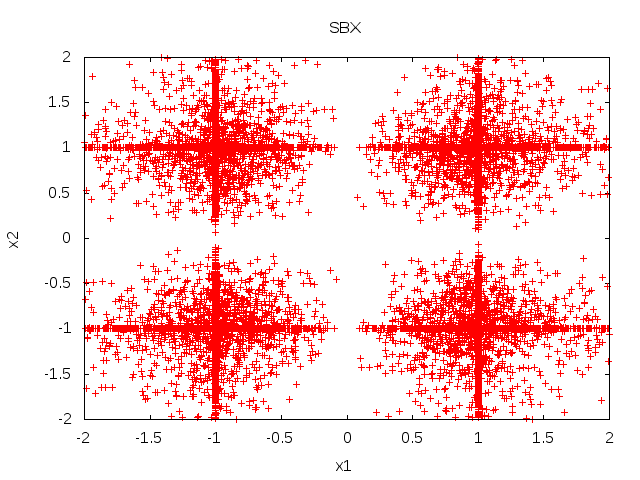
\includegraphics[width=0.24\textwidth]{img/Operadores/SBX_eta_2.png}  %&
   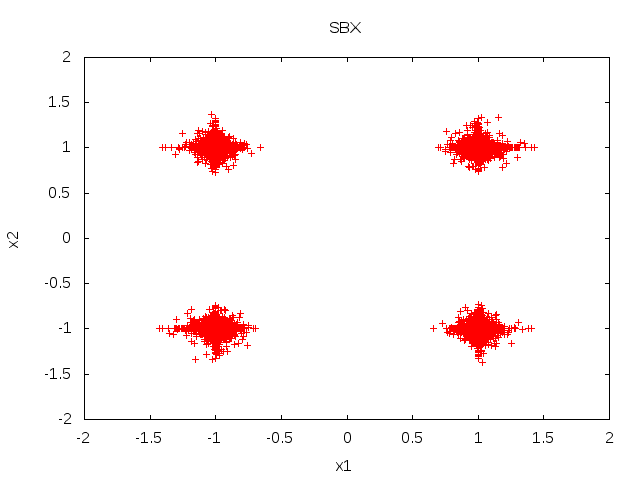
\includegraphics[width=0.24\textwidth]{img/Operadores/SBX_eta_20.png} 
\end{tabular}
\caption{Simulation of the \SBX{} operator sampling $10,000$ children values, the parents are located in $P_1=(-1.0, -1.0)$ and $P_2=(1.0, 1.0)$. The left and right are with a distribution index of $2$ and $20$ respectively.}
\label{fig:Simulation_Case_3}
\end{figure}

El segundo aspecto clave es después de generar dos valores de las soluciones hijo con la distribución \SBX{}, ya que estos valores son intercambiados con una probabilidad fija que usualmente es $0.5$, es decir el valor de la solución hijo $c_1$ no siempre es heradado por la solución padre mas cercana $p_1$.
%The second key issue is that after generating the two child values with the \SBX{} distribution, such values
%are interchanged with a fixed probability that is usually set to $0.5$, i.e. the value closer to parent $p_1$ is
%not always inherited by $c_1$.
%
Esta es una característica no muy discutida, sin embargo es un aspecto muy relevante y afecta al rendimiento del algoritmo.
%This is a feature that is not usually discussed but it is important for the obtained performance.
%
En algunos contextos esta probabilidad se identifica como ``Probabilidad de cruce uniforme por variable'' (Variable uniform crossover probability) \cite{tuvsar2007differential} o ``Recombinación Discreta'' (Discrete Recombination) \cite{muhlenbein1993predictive}.

%In some contexts this probability is known as ``Variable uniform crossover probability'' 
%\cite{tuvsar2007differential} or ``Discrete Recombination'' \cite{muhlenbein1993predictive}.
%
Desde que en el ámbito multi-objetivo se promueve más diversidad en las variables de decision de forma implícita, estos intercambios podrían ser altamente disruptivos.
%Since in multi-objective optimization more diversity is maintained these swaps might produce a high disruptive operator.
%
De hecho, en algún sentido y dado a esto, no es totalmente claro que el \SBX{} pueda ser categorizado como un operador totalmente basado en los padres.
%In fact, in some sense due to this action it is not so clear that \SBX{} can be categorized as a parent-centric operator.
%
Estos intercambios que existen entre los valores de las soluciones hijo tienen un efecto de realizar múltiples ``reflexiones'' en el espacio de búsqueda.
%These interchanges between the children has the effect of performing multiple ``reflections'' in the search space.
%
De hecho, conforme incrementa la dimensionalidad en el espacio de las variales, el número de regiones cubiertas incrementa de forma exponencial como se puede observar en los casos de dos y tres dimensiones en la figura \ref{fig:Simulations_Index_20}.
%When increasing the dimensions of the decision variables the number of regions covered increases exponentially 
%as is illustrated in Figure \ref{fig:Simulations_Index_20} where cases with two and three decision variables are taken into account.
%
Es importante notar que esta característica tiene un efecto relevante en la distancia entre las soluciones padre y las soluciones hijo.
%Note also that this feature has a considerable effect on the distance between parents and offspring.

Finalmente, siendo quizás la característica mas conocida del operador \SBX{} es el índice de distribución.
%Finally, the last component is the distribution index, which is probably the most well known feature of the \SBX{}.
%
Un índice de distribución pequeño provoca un grado de exploración elevado.
%A low index results in greater exploration levels.
%
De hecho, un índice de distribución de la unidad tiene un efecto similar al \textit{Operador de Recombinación Difusa} (Fuzzy Recombination Operator) \cite{voigt1995fuzzy}.
%In fact, a distribution index equal to one has a similar effect to the Fuzzy Recombination Operator \cite{voigt1995fuzzy}.
%
En la figura~\ref{fig:Simulation_Case_3} se puede observar el efecto de aplicar distintos índices de distribución.
%
Particularmente, en la parte izquierda se considera un índice de distribución pequeño, mientras en la parte derecha se considera un índice de distribución grande, se observa que este último genera soluciones candidatas similares a las soluciones padre.
%The effect of applying different indexes is illustrated in Figure~\ref{fig:Simulation_Case_3} where the left side
%considers a low index value whereas the right side takes into account a higher index value, which creates 
%new candidate solutions that are more similar to the parents.
%

En el algoritmo \ref{alg:SBX_Operator} se muestra la implementación del operador \SBX{}.
%The \SBX{} implementation is shown in Algorithm \ref{alg:SBX_Operator}.
%
Este pseudocódigo está basado en la implementación que está integrado en el código \NSGAII propuesto por Deb y otros \cite{Joel:NSGAII}, el cual es considerada como la variante mas popular.
%This pseudocode is based on the implementation that is integrated in the NSGA-II code published by Deb et al. \cite{Joel:NSGAII} and which
%is the most popular variant nowadays.
%
Como parámetros de entrada se requieren dos soluciones padre ($P_1$ and $P_2$), y como salida se obtinen dos soluciones hijo ($C_1$ and $C_2$).
%As an input it requires two parents ($P_1$ and $P_2$) and it creates two children ($C_1$ and $C_2$).
%
El primero y el segundo componente que mencionados previamente corresponden a las líneas 5 y 9 respectivamente.
%The first and second key components commented previously correspond to the lines 5 and 8, respectively. 
%
Como es usual, el caso clásico del operador \SBX{} es configurado asignando los parámetros $\delta_1 = \delta_2 = 0.5$ y $\eta_c = 20$.
%As is usual, for the basic case, \SBX{} is configured with $\delta_1 = \delta_2 = 0.5$ and $\eta_c = 20$.
%
Es important notar que la implementación clásica no considera la dimensión de la variable o el criterio de paro en sus parámetros internos.
%It is important take into account that this implementation does not consider the dimension of the decision variables 
%or the stopping criteria to set any of its internal parameters.

\subsection{Propuesta}

Basado en el análisis anterior y con el propósito de inducir un balance entre exploración e intensificación, se proponen las siguiente modificaciones.
%Based on the previous analyses and with the aim of inducing an appropriate balance between 
%exploration and intensification, the following modifications are proposed.
%
Primeramente, se modifica la probabilidad de alterar una variable ($\delta_1$) durante la ejecución de forma dinámica.
%First, the probability to modify a variable ($\delta_1$) is dynamically
%modified during the execution.
%
La intención de esta modificación es incrementar la capacidad de exploración en las primeras etapas, esto alterando de forma simultánea un conjunto de variables y conforme la execución procede se reduce el número de variables que son modificadas.
%The rationality behind this modification is to increase the exploration capability in the initial stages
%by altering simultaneously several variables and then, as the evolution proceeds reduce the number of variables
%that are modified.
%
El valor de $\delta_1$ se cambia en base a un modelo lineal decreciente, donde inicialmente es fijado a $1.0$ y entonces es decrementado hasta la mitad del total de generaciones con un valor de $0.5$.
%The value of $\delta_1$ is changed in base of a linear decreasing model, where initially it is fixed to $1.0$ and 
%then it is decreased so that at the half of total generations is equal to $0.5$.
%
Esta último valor es mantenido haste el final de la ejecución, es decir desde la mitad de la execución este parámetro se comporta similar a la implementación tradicional del \SBX{}.
%This last value is maintained until the end of the execution, i.e. from the half of the execution it behaves as the 
%traditional \SBX{} implementation.
%

Para asignar el valor $\delta_1$ se utiliza la ecuación (\ref{eqn:linear}), donde $G_{Transcurridas}$ corresponde a la generación actual y $G_{Total}$ corresponde al número total de generaciones.
%Equation (\ref{eqn:linear}) is the one used to set the value of $\delta_1$, where $G_{Elapsed}$ is the current generation 
%and $G_{End}$ is the total number of generations.

Similarmente, el segundo cambio está relacionado con la probabilidad de aplicar reflexiones ($1 - \delta_2$).
%In a similar way, the second change is related to the probability of performing reflections ($1 - \delta_2$).
%
En este caso $\delta_2$ es actualizado de acuerdo a la ecuación (\ref{eqn:linear}), por lo tanto la probabilidad de aplicar una reflexión incrementa de $0.0$ a $0.5$ durante la ejecución.
%In this case $\delta_2$ is also updated as in Equation (\ref{eqn:linear}), meaning that the probability of performing
%a reflection increases from $0.0$ to $0.5$ during the execution.
%
Esta modificación se realiza con el propósito de evitar el comportamiento disruptivo de intercambiar variables en las primeras generaciones ya que esto provocaría modificaciones muy drásticas.
%This modification is performed with the aim of avoiding the disruptive behavior of interchanging the variables at the
%first generations because this might result in very drastic modifications.
%
De esta forma, sería mas sensato aplicar estas reflexiones una vez que los individuos convergen a cierto grado-
%Once that the individuals converge to certain degree it might make more sense to perform such reflections.
%
Por lo tanto, esta probabilidad es incrementado a $0.5$, siendo el valor utilizando en la implementación del \SBX{} estándar.
%Thus, this probability is increased to $0.5$ which is the value used in the standard implementation of \SBX{}.

\begin{equation}\label{eqn:linear}
	\delta_1 = \delta_2 = max \left (0.5, 1.0 - \frac{G_{Transcurridas}}{G_{Total}} \right )
\end{equation}

Finalmente, el índice de distribución también es modificado durante la ejecución.
%Finally, the distribution index is also changed during the execution. 
%
De esta forma, en la primeras etapas se promueve un íncide de distribución pequeño con el propósito de incrementar la capacidad de exploración del \SBX{}.
%At the first stages a low distribution index is induced with the aim of increasing the exploration capabilities 
%of \SBX{}.
%
Posteriormente es decrementado de forma lineal, lo cual tiene implica que la curva de distribución se cierre, por lo tanto se promueve un mayor grado de intensificación en las etapas finales.
%Then, it is linearly incremented which has the effect of closing the distribution curve, meaning that more intensification is
%promoted.
%
El incremento lineal es indicado en la ecuación (\ref{eqn:index_eta}), por lo tanto el índice de distribución es alterado de $2$ a $22$.
%The linear increment is governed by Equation (\ref{eqn:index_eta}), meaning that the distribution index is altered
%from $2$ to $22$.
%
Es importante hacer mención que ya se han considerado modificaciones similares al índice de distribución \cite{zitzler1999multiobjective}, \cite{hamdan2012distribution}.
%Note that modifications similar to this last one have been explored previously 
%\cite{zitzler1999multiobjective}, \cite{hamdan2012distribution}.
%

\begin{equation}\label{eqn:index_eta}
 \eta_c = 2 + 20 \times \left ( \frac{G_{Elapsed}}{G_{End}} \right)
\end{equation}

\subsection{Resultados}

\begin{table}[t]
\centering
\scriptsize
\caption{Puntos de referencias para el indicador HV}
%\caption{References points for the HV indicator}
\label{tab:ReferencePoints}
\begin{tabular}{cc}
\hline
\textbf{Instancias} & \textbf{Punto de referencia} \\ \hline
%\textbf{Instances} & \textbf{Reference Point} \\ \hline
WFG1-WFG9 & $[2.1, ...,2m+0.1]$ \\
DTLZ 1, 2, 4 & $[1.1, ..., 1.1]$ \\
DTLZ 3, 5, 6 & $[3, ..., 3]$ \\
DTLZ7 & $[1.1, ..., 1.1, 2m]$ \\
UF 1-10 & $[2, ..., 2]$ \\ \hline
\end{tabular}
\end{table}


% Please add the following required packages to your document preamble:
% \usepackage{multirow}
% \usepackage{graphicx}
\begin{table*}[t]
\centering

\caption{Información estadística de las métricas considerando dos objetivos}
%\caption{Statistical Information of Metrics with two objectives}
\label{tab:Metrics_2}
\resizebox{\textwidth}{!}{%
\begin{tabular}{|c|c|c|c|c|c|c|c|c|c|c|c|c|c|c|c|c|c|c|}
\hline
\multirow{2}{*}{} & \multicolumn{6}{c|}{NSGA-II} & \multicolumn{6}{c|}{MOEA/D} & \multicolumn{6}{c|}{SMS-EMOA} \\ \cline{2-19} 
 & 1 & 2 & 3 & 4 & 5 & DE & 1 & 2 & 3 & 4 & 5 & DE & 1 & 2 & 3 & 4 & 5 & DE \\ \hline
Average HV & 0.88 & 0.90 & 0.90 & 0.91 & 0.93 & \textbf{0.94} & 0.87 & 0.87 & 0.87 & 0.90 & \textbf{0.91} & \textbf{0.91} & 0.88 & 0.89 & 0.87 & 0.91 & 0.92 & \textbf{0.93} \\ \hline
%Best Counts HV & 2 & 1 & 0 & 1 & 8 & \textbf{11} & 2 & 0 & 2 & 2 & 8 & \textbf{9} & 0 & 1 & 1 & 5 & 6 & \textbf{10} \\ \hline
%\multicolumn{1}{|l|}{Average Best Difference HV} & \multicolumn{1}{l|}{0.068} & \multicolumn{1}{l|}{0.057} & \multicolumn{1}{l|}{0.053} & \multicolumn{1}{l|}{0.039} & \multicolumn{1}{l|}{0.019} & \multicolumn{1}{l|}{\textbf{0.017}} & \multicolumn{1}{l|}{0.053} & \multicolumn{1}{l|}{0.048} & \multicolumn{1}{l|}{0.049} & \multicolumn{1}{l|}{0.024} & \multicolumn{1}{l|}{\textbf{0.013}} & \multicolumn{1}{l|}{0.014} & \multicolumn{1}{l|}{0.074} & \multicolumn{1}{l|}{0.064} & \multicolumn{1}{l|}{0.081} & \multicolumn{1}{l|}{0.045} & \multicolumn{1}{l|}{0.028} & \multicolumn{1}{l|}{\textbf{0.019}} \\ \hline
Average IGD+ & 0.12 & 0.09 & 0.11 & 0.07 & 0.06 & \textbf{0.05} & 0.14 & 0.12 & 0.14 & 0.09 & 0.08 & \textbf{0.07} & 0.13 & 0.11 & 0.14 & 0.08 & 0.07 & \textbf{0.05} \\ \hline
%Best Counts IGD+ & 2 & 1 & 1 & 1 & 8 & \textbf{10} & 3 & 0 & 2 & 3 & 6 & \textbf{9} & 0 & 2 & 0 & 3 & \textbf{9} & \textbf{9} \\ \hline
%\multicolumn{1}{|l|}{Average Best Difference IGD+} & \multicolumn{1}{l|}{0.086} & \multicolumn{1}{l|}{0.052} & \multicolumn{1}{l|}{0.077} & \multicolumn{1}{l|}{0.035} & \multicolumn{1}{l|}{0.021} & \multicolumn{1}{l|}{\textbf{0.016}} & \multicolumn{1}{l|}{0.075} & \multicolumn{1}{l|}{0.059} & \multicolumn{1}{l|}{0.072} & \multicolumn{1}{l|}{0.025} & \multicolumn{1}{l|}{0.019} & \multicolumn{1}{l|}{\textbf{0.008}} & \multicolumn{1}{l|}{0.093} & \multicolumn{1}{l|}{0.071} & \multicolumn{1}{l|}{0.101} & \multicolumn{1}{l|}{0.038} & \multicolumn{1}{l|}{0.030} & \multicolumn{1}{l|}{\textbf{0.017}} \\ \hline
\end{tabular}%
}
\end{table*}

% Please add the following required packages to your document preamble:
% \usepackage{multirow}
% \usepackage{graphicx}
\begin{table*}[t]
\centering
\caption{Información estadística de las métricas considerando tres objetivos}
%\caption{Statistical Information of Metrics with three objectives}
\label{tab:Metrics_3}
\resizebox{\textwidth}{!}{%
\begin{tabular}{|c|c|c|c|c|c|c|c|c|c|c|c|c|c|c|c|c|c|c|}
\hline
\multirow{2}{*}{} & \multicolumn{6}{c|}{NSGA-II} & \multicolumn{6}{c|}{MOEA/D} & \multicolumn{6}{c|}{SMS-EMOA} \\ \cline{2-19} 
 & 1 & 2 & 3 & 4 & 5 & DE & 1 & 2 & 3 & 4 & 5 & DE & 1 & 2 & 3 & 4 & 5 & DE \\ \hline
Average HV & \textbf{0.87} & 0.84 & \textbf{0.87} & \textbf{0.87} & \textbf{0.87} & 0.85 & 0.84 & 0.84 & 0.84 & \textbf{0.86} & \textbf{0.86} & 0.85 & 0.90 & 0.89 & 0.88 & \textbf{0.91} & \textbf{0.91} & \textbf{0.91} \\ \hline
%Best Counts HV & 1 & 2 & 1 & 4 & 4 & \textbf{7} & 1 & 2 & 1 & 2 & 5 & \textbf{8} & 3 & 2 & 0 & 2 & 5 & \textbf{7} \\ \hline
%\multicolumn{1}{|l|}{Average Best Difference HV} & \multicolumn{1}{l|}{0.019} & \multicolumn{1}{l|}{0.047} & \multicolumn{1}{l|}{0.020} & \multicolumn{1}{l|}{\textbf{0.014}} & \multicolumn{1}{l|}{\textbf{0.014}} & \multicolumn{1}{l|}{0.032} & \multicolumn{1}{l|}{0.036} & \multicolumn{1}{l|}{0.041} & \multicolumn{1}{l|}{0.038} & \multicolumn{1}{l|}{0.016} & \multicolumn{1}{l|}{\textbf{0.013}} & \multicolumn{1}{l|}{0.027} & \multicolumn{1}{l|}{0.038} & \multicolumn{1}{l|}{0.038} & \multicolumn{1}{l|}{0.049} & \multicolumn{1}{l|}{\textbf{0.019}} & \multicolumn{1}{l|}{0.027} & \multicolumn{1}{l|}{\textbf{0.019}} \\ \hline
Average IGD+ & 0.13 & 0.16 & 0.13 & \textbf{0.12} & \textbf{0.12} & 0.13 & 0.15 & 0.14 & 0.15 & \textbf{0.11} & \textbf{0.11} & 0.13 & 0.11 & 0.11 & 0.13 & \textbf{0.09} & \textbf{0.09} & 0.13 \\ \hline
%Best Counts IGD+ & 0 & 2 & 2 & 4 & 3 & \textbf{8} & 2 & 2 & 0 & 2 & 4 & \textbf{9} & 1 & 3 & 0 & 3 & 5 & \textbf{7} \\ \hline
%\multicolumn{1}{|l|}{Average Best Difference IGD+} & \multicolumn{1}{l|}{0.029} & \multicolumn{1}{l|}{0.061} & \multicolumn{1}{l|}{0.027} & \multicolumn{1}{l|}{0.023} & \multicolumn{1}{l|}{\textbf{0.020}} & \multicolumn{1}{l|}{0.032} & \multicolumn{1}{l|}{0.053} & \multicolumn{1}{l|}{0.048} & \multicolumn{1}{l|}{0.053} & \multicolumn{1}{l|}{\textbf{0.015}} & \multicolumn{1}{l|}{\textbf{0.015}} & \multicolumn{1}{l|}{0.030} & \multicolumn{1}{l|}{0.047} & \multicolumn{1}{l|}{0.040} & \multicolumn{1}{l|}{0.062} & \multicolumn{1}{l|}{\textbf{0.020}} & \multicolumn{1}{l|}{0.024} & \multicolumn{1}{l|}{0.069} \\ \hline
\end{tabular}%
}
\end{table*}
\begin{table*}[t]
\centering
\caption{Resúmen de las pruebas estadísticas}
%\caption{Summary of Statistical Tests}
\label{tab:statistical_Tests}
\begin{tabular}{|c|c|c|c|c|c|c|c|c|c|c|c|c|c|c|c|}
\hline
\multicolumn{16}{|c|}{NSGA-II} \\ \hline
 & \multicolumn{3}{c|}{1} & \multicolumn{3}{c|}{2} & \multicolumn{3}{c|}{3} & \multicolumn{3}{c|}{4} & \multicolumn{3}{c|}{5} \\ \hline
 & $\uparrow$ & $\downarrow$ & $\longleftrightarrow$ & $\uparrow$ & $\downarrow$ & $\longleftrightarrow$ & $\uparrow$ & $\downarrow$ & $\longleftrightarrow$ & $\uparrow$ & $\downarrow$ & $\longleftrightarrow$ & $\uparrow$ & $\downarrow$ & $\longleftrightarrow$ \\ \hline
\textbf{HV-2obj} & 16 & 29 & 47 & 6 & 61 & 25 & 28 & 19 & 45 & 31 & 23 & 38 & \textbf{54} & 3 & 35 \\ \hline
\textbf{HV-3obj} & 15 & 19 & 42 & 12 & 50 & 14 & 17 & 15 & 44 & \textbf{33} & 10 & 33 & 26 & 9 & 41 \\ \hline
\textbf{IGD-2obj} & 14 & 30 & 48 & 4 & 60 & 28 & 25 & 17 & 50 & 33 & 19 & 40 & \textbf{52} & 2 & 38 \\ \hline
\textbf{IGD-3obj} & 14 & 18 & 44 & 13 & 44 & 19 & 18 & 15 & 43 & \textbf{33} & 15 & 28 & 23 & 9 & 44 \\ \hline
% \end{tabular}
% \end{table*}

% \begin{table*}[]
% \centering
% \caption{My caption}
% \label{my-label}
% \begin{tabular}{|c|c|c|c|c|c|c|c|c|c|c|c|c|c|c|c|}
\hline
\hline
\multicolumn{16}{|c|}{MOEA/D} \\ \hline
 & \multicolumn{3}{c|}{1} & \multicolumn{3}{c|}{2} & \multicolumn{3}{c|}{3} & \multicolumn{3}{c|}{4} & \multicolumn{3}{c|}{5} \\ \hline
 & $\uparrow$ & $\downarrow$ & $\longleftrightarrow$ & $\uparrow$ & $\downarrow$ & $\longleftrightarrow$ & $\uparrow$ & $\downarrow$ & $\longleftrightarrow$ & $\uparrow$ & $\downarrow$ & $\longleftrightarrow$ & $\uparrow$ & $\downarrow$ & $\longleftrightarrow$ \\ \hline
\textbf{HV-2obj} & 15 & 33 & 44 & 10 & 60 & 22 & 25 & 26 & 41 & 39 & 18 & 35 & \textbf{57} & 9 & 26 \\ \hline
\textbf{HV-3obj} & 10 & 22 & 44 & 12 & 39 & 25 & 11 & 19 & 46 & 24 & 10 & 42 & \textbf{38} & 5 & 33 \\ \hline
\textbf{IGD-2obj} & 16 & 31 & 45 & 9 & 60 & 23 & 23 & 27 & 42 & 37 & 17 & 38 & \textbf{57} & 7 & 28 \\ \hline
\textbf{IGD-3obj} & 12 & 22 & 42 & 13 & 43 & 20 & 13 & 24 & 39 & 30 & 9 & 37 & \textbf{40} & 10 & 26 \\ \hline
% \end{tabular}
% \end{table*}

% \begin{table*}[]
% \centering
% \caption{My caption}
% \label{my-label}
% \begin{tabular}{|c|c|c|c|c|c|c|c|c|c|c|c|c|c|c|c|}
\hline
\hline
\multicolumn{16}{|c|}{SMS-EMOA} \\ \hline
 & \multicolumn{3}{c|}{1} & \multicolumn{3}{c|}{2} & \multicolumn{3}{c|}{3} & \multicolumn{3}{c|}{4} & \multicolumn{3}{c|}{5} \\ \hline
 & $\uparrow$ & $\downarrow$ & $\longleftrightarrow$ & $\uparrow$ & $\downarrow$ & $\longleftrightarrow$ & $\uparrow$ & $\downarrow$ & $\longleftrightarrow$ & $\uparrow$ & $\downarrow$ & $\longleftrightarrow$ & $\uparrow$ & $\downarrow$ & $\longleftrightarrow$ \\ \hline
\textbf{HV-2obj} & 9 & 35 & 48 & 7 & 43 & 42 & 16 & 31 & 45 & 41 & 9 & 42 & \textbf{53} & 8 & 31 \\ \hline
\textbf{HV-3obj} & 7 & 21 & 48 & 9 & 35 & 32 & 13 & 21 & 42 & 27 & 6 & 43 & \textbf{31} & 4 & 41 \\ \hline
\textbf{IGD-2obj} & 10 & 34 & 48 & 15 & 48 & 29 & 12 & 33 & 47 & 41 & 12 & 39 & \textbf{55} & 6 & 31 \\ \hline
\textbf{IGD-3obj} & 8 & 20 & 48 & 13 & 30 & 33 & 9 & 19 & 48 & 22 & 5 & 49 & \textbf{27} & 5 & 44 \\ \hline
\end{tabular}
\end{table*}

En este apartado se analizan los resultados obtenidos con las variantes dinámicas del \SBX{} (\DSBX{}).
%This section is devoted to analyze the results obtained with the dynamic variants of \SBX{} (\DSBX{}).
%
Cada uno de los casos estudiados y una propuesta final se integraron en los algoritmos \NSGAII{}, \MOEAD{} and \SMSEMOA{}.
%The novel crossover operator was integrated with \NSGAII{}, \MOEAD{} and \SMSEMOA{}.
%
Primeramente, es analizado cada uno de los tres componentes previamente analizados.
%First, three variants that alter only one of each of the components previously discussed are analyzed.
%
Posteriormente se construye un caso donde se consideran dos componentes de forma simultánea.
%Then, a case that alters two of them simultaneously is taken into account.
%
%%##UNFINISHED
Se consideran los problemas de prueba WFG \cite{Joel:WFG}, DTLZ \cite{Joel:DTLZ_2} and UF \cite{zhang2009performance}.
%The WFG \cite{Joel:WFG}, DTLZ \cite{Joel:DTLZ_2} and UF \cite{zhang2009performance} test problems have been used for our purpose.
%
Con el propósito de comparar nuestra extensión del \SBX{} con otros operadores populares en la validación experimental incluímos una variante de evolución diferencial mejor conocida como \DEMO{}~\cite{tuvsar2007differential}.
%Our experimental validation also includes the variant of Differential Evolution known as DEMO~\cite{tuvsar2007differential}
%with the aim of comparing our extension of \SBX{} with other well-known operators.
Debido a que todos los algoritmos con estocástico cada ejecución se repitió $35$ veces con distintas semilla 
%Given that all the methods are stochastic algorithms, each execution was repeated $35$ times with different seeds.
%
La configuración global que es aplicada a todos los algoritmos es como es indica a continuación.
%
Se asgina el criterio de paro a $25,000$ generaciones, el tamaño de la población a $100$, se configuraron los problemas de prueba \WFG{} con dos y tres objetivos, además se consideraron 24 variables, donde $20$ variables eran considerados como parámetros de distancia y $4$ se consideraron como parámetros de posición.
%The common configuration in all of them was the following: the stopping criterion was set to $25,000$ generations, 
%the population size was fixed to 100, WFG test problems were configured with two and three objectives, and 24 variables
%were considered, where 20 of them are distance parameters and 4 of them are position parameters.
%
Como es sugerido en \cite{Joel:DTLZ_2} se consideran $n=M+r-1$ variables de decisión en los problemas de prueba \DTLZ{}, donde para los problemas DTLZ1, DTLZ2 - DTLZ6 y DTLZ7 se consideraron $r=\{5, 10, 20\}$  respectivamente.
%In the case of the DTLZ test instances, the number of decision variables were set to $n=M+r-1$, where $r=\{5, 10, 20\}$ 
%for DTLZ1, DTLZ2 to DTLZ6 and DTLZ7 respectively, as is suggested in\cite{Joel:DTLZ_2}.  
% 
Para los problemas de prueba \UF{} se asignaron $10$ variable de decisión.
%In the UF benchmark set the number of decision variables were set to 10.
%
Finalmente, se asignó al operador de mutación polinomial con una probabilidad de cruce de $1/n$ y con un índice de distribución de $50$, mientras que el operador de cruce \SBX{} se asignó con una probabilidad de cruce de $0.9$ y un índice de distribución de $20$.
%Finally, the polynomial mutation was used with a mutation probability equal to $1/n$ and with a distribution index equal to 50, 
%whereas for the cases that used the \SBX{}, the crossover probability was set to $0.9$ and the distribution index
%was set to 20.
%
A continuación se especifica la parametrización adicionel de cada algoritmo:
%The additional parameterization of each algorithm was as follows:
\begin{itemize}
\item \textbf{DEMO}: CR = 0.3 and F = 0.5.
\item \textbf{SMS-EMOA}: desplazamiento para calcular el HV = 100.
%\item \textbf{SMS-EMOA}: offset = 100.
\item \textbf{MOEA/D}: tamaño de la vecindad = 10, el número de actualizaciones por subproblema ($nr$) = 2 y $\delta = 0.9$.
i%\item \textbf{MOEA/D}: size of neighborhood = 10, max updates by sub-problem (nr) = 2 and $\delta = 0.9$.
\end{itemize}

Para comparar los frentes obtenidos de cada método se utiliza el hipervolúmen normalizado (HV) y la \textit{Distanca Generacional Invertida Modificada} (Inverted Generational Distance Plus - IGD+).
%In order to compare the fronts obtained by the different methods the 
%normalized hypervolume (HV) and IGD+ was taken into account.
%
En la tabla \ref{tab:ReferencePoints} se presentan los puntos de referencia utilizados para el indicador del hipervolúmen los cuales son similares a los utilizados en \cite{Joel:Kuhn_Munkres, Joel:OperatorAHX}.
%The reference points used for the hypervolume indicator are shown in the Table \ref{tab:ReferencePoints} 
%and are similar to the ones used in \cite{Joel:Kuhn_Munkres, Joel:OperatorAHX}.
%
Por otra parte para comparar los resultados estadísticamente (valores del IGD+ y HV), se siguió un procedimiento similar al que se propuso en~\cite{Joel:StatisticalTest}.
%In order to statistically compare the results (IGD+ and HV values), the following statistical tests were performed. 
%In order to statistically compare the results, a similar guideline than the one proposed in~\cite{Joel:StatisticalTest} was used. 
%
En primer lugar se utilizó el test Shapiro-Wilk para comprobar si los resultados se ajustaban a una distribución Gaussiana. 
%
%First a Shapiro-Wilk test was performed to check whatever or not the values of the results followed a Gaussian distribution. 
%
%En los casos en que sí se ajustaban, se utilizó el test de Levene para comprobar la homogeneidad de las varianzas, procediendo con el test de ANOVA en caso positivo o con el de Welch en caso negativo.
%
%If, so, the Levene test was used to check for the homogeneity of the variances. 
%If samples had equal variance, an ANOVA test was done; if not, a Welch test was performed. 
%
Por otro lado, para los casos que no se ajustaban a distribuciones Guassianas, se utilizó el test de Kruskal-Wallis.
%For non-Gaussian distributions, the nonparametric Kruskal-Wallis test was used to test whether samples are drawn 
%from the same distribution. 
%
En todos los casos se fijó el nivel de confianza al 95\%.
%
Se considera que un algoritmo $X$ es superior a un algoritmo $Y$, si el procedimiento anterior reporta diferencias significativas y si la media y mediana del hipervolumen obtenido por el método $X$ son superiores a las obtenidas por el método $Y$.
%
%An algorithm $X$ is said to win algorithm $Y$ when the differences between them are statistically significant, and
%the mean and median obtained by $X$ are higher (in HV) or lower (in IGD+) than the mean and median achieved by $Y$.


\subsection{Análisis de cada compenente en el operador \SBX{}}
%\subsection{Analysis of isolated components}

En este apartado se analiza el efecto que cada componente tiene de forma independente al ser dinámicamente modificado
%In this section we discuss about the independent effect of each component that is dynamically modified.
%
%
Basados en el algoritmo \ref{alg:SBX_Operator} el efecto de cada componente es analizado a través de cuatro casos
%The effect of each component is analyzed through four cases, based in the Algorithm \ref{alg:SBX_Operator}.
%
Cada caso es descrito a continuación.
%Each case is described as follows:

\begin{itemize}
\item \textbf{Caso 1}: Se aplica la versión estańdar del operador \SBX{} donde $\delta_1 = \delta_2 = 0.5$ y $\eta_c = 20$.
%\item \textbf{Case 1}: The standard SBX operator where $\delta_1 = \delta_2 = 0.5$ and $\eta_c = 20$.
\item \textbf{Caso 2}: Se actualiza el valor $\delta_1$ como se indica en la ecuación~(\ref{eqn:linear}),  $\delta_2=0.5$ y $\eta_c = 20$.
%\item \textbf{Case 2}: The value $\delta_1$ is updated according to Equation~(\ref{eqn:linear}),  $\delta_2=0.5$ and $\eta_c = 20$.
\item \textbf{Caso 3}: Se actualiza el valor $\delta_2$ como se indica en la ecuación~(\ref{eqn:linear}), $\delta_1=0.5$ y $\eta_c = 20$.
%\item \textbf{Case 3}: The value $\delta_2$ is updated according to Equation~(\ref{eqn:linear}), $\delta_1=0.5$ and $\eta_c = 20$.
\item \textbf{Caso 4}: Se actualiza el índice de distribución de acuerdo a~(\ref{eqn:index_eta}), $\delta_1=\delta_2=0.5$.
%\item \textbf{Case 4}: The distribution index is updated according to Equation~(\ref{eqn:index_eta}), $\delta_1=\delta_2=0.5$.
\end{itemize}

En las tablas \ref{tab:Metrics_2} y \ref{tab:Metrics_3} se muestra información del HV normalizado \cite{zitzler1999multiobjective} y del IGD+ \cite{Joel:IGDPlus_And_GDPlus} para cada caso (Posteriormente se analiza el Caso 5).
%In order to analyze the performance of each Case (Case 5 is discussed later), Tables \ref{tab:Metrics_2} and
%\ref{tab:Metrics_3} shows information about the Normalized Hyper-volume 
%(HV)~\cite{zitzler1999multiobjective} and about the Inverted Generational Distance Plus (IGD+)~\cite{Joel:IGDPlus_And_GDPlus}.
%
Específicamente, se muestra la media del HV e IGD+ para todos los problemas en dos y tres objetivos.
%Specifically, the mean of the HV and IGD+ for all considered problems are shown for two and three objectives.
%
Se observa que considerando dos y tres objetivos el Caso 4 mejora al Caso 1, al Caso 2 y al Caso 3 en todos los algoritmos.
%It is clear that case 4 outperforms case 1, case 2 and case 3 both with two and three objectives in all the tested algorithms.
%
Por lo tanto se aprecian los beneficios de incrementar el índice de distribución durante la ejecución.
%%Therefore, increasing the distribution index during the execution seems to be the most beneficial action.
%
Esto sucede porque inicialmente la curva que corresponde a la distribución de probabilidad conduce a un grado elevado de exploración, mientras que al trancurrir las generaciones se cambia gradualmente a un procedo de intensificación.
%This occurs because the initially open distribution curve leads to a higher degree of exploration, whereas as the evolution
%proceeds more intensification is promoted.
%
Por otra parte, al considerar tres objetivos el Caso 2 presentó un rendimiento menor que al Caso 1.
%On the other hand, case 2 presented a lower performance than case 1 when taking into account three objectives.
%
Por lo tanto, se observa que alterar todas las variables provoca un comportamiento muy disruptivo.
%Thus, it seems that altering almost all the variables convert the new approach into a too disruptive operator.
%
Quizás los resultados podrían mejorar si el parámetro $\delta_1$ es alterado de una forma distinta, sin embargo esto se deja como trabajo futuro.
%Perhaps, altering $\delta_1$ in a different way might provide better results, but this is left as a future work.
Los análisis anteriores únicamente consideran la media obtenida en todos los problemas de prueba.
%Previous analyses are only based on the mean obtained for all the problems.
%
Sin embargo, dependiendo en el tipo de problema el rendimiento del algoritmo podría cambiar.
%However, depending on the problem the performance might vary.
%
Esto se analiza en la siguiente sección.
%This is analyzed in the following section.
%
Adicionalmente, se anexan resultados detallados\footnote{https:\//\//github.com\//joelchaconcastillo\//SBX\_CEC2018.}.
%Additionally, more detailed results are available\footnote{https:\//\//github.com\//joelchaconcastillo\//SBX\_CEC2018.}.


\subsection{Modificación simiultánea de varios componentes}
%\subsection{Simultaneous modification of several components}

En base a los resultados obtenidos con anterioridad se propone una variante del operador \SBX{}.
%
En esta variante se considera el Caso 3 y el Caso 4 de forma simultánea, es decir existen un cambio dinámico en el parámetro $\delta_2$ y en el índice de distribución.
%Based on the previously discussed results, a variant of the \SBX{} is proposed where the case 3 and case 4 are mixed, 
%i.e. both $\delta_2$ and the distribution index are updated dynamically.
%
El Caso 2 donde se aplica un mecanismo para actualiza $\delta_1$ no se considera debido que los beneficios con esta variante no fueron significativos.
%Since case 2 did not report significant benefits, the updating mechanism for $\delta_1$ was discarded.
%
Particularmente, el Caso 5 es construido en base al Algoritmo \ref{alg:SBX_Operator} y es configurado como se indica a continuación.
%Specifically in our case 5, Algorithm \ref{alg:SBX_Operator} is configured as follows.
%
El parámetro $\delta_1$ es asignado con $0.5$ ya que es la forma de la versión estándar del \SBX{}.
%The parameter $\delta_1$ is fixed to $0.5$, i.e. in a similar way than the standard \SBX{}.
%
En base al Caso 3, el parámetro $\delta_2$ es actualizado de acuerdo a la ecuación~(\ref{eqn:linear}).
%Following the case 3, $\delta_2$ is updated according to Equation~(\ref{eqn:linear}).
%
Finalmente, en base al Caso 4, el parámetro $\delta_2$ es actualizado como se indica en la ecuación (\ref{eqn:index_eta}).
%Finally, according to case 4 $\eta_c$ is updated in base of Equation~(\ref{eqn:index_eta}).

De acuerdo a la media del HV y del IGD+ que se obtuvieron en el Caso 5 (revisar tablas~\ref{tab:Metrics_2} and \ref{tab:Metrics_3}), se pueden observar los beneficios de integrando los Casos 3 y 4.
%Attending to the mean HV and IGD+ obtained by the case 5 (see Tables~\ref{tab:Metrics_2} and \ref{tab:Metrics_3})
%it is clear that integrating case 3 and case 4 is beneficial.
%
En el caso de dos objetivos se observa una ventaja significativa, sin embargo en el caso de tres objetivo los Casos 4 y 5 son muy similares en base a la media.
%The advantages are clearer in the case of two objectives, whereas in the case of three objectives, case 4
%and case 5 are similar in terms of mean performance.
%
Además, al considerar tres objetivos los resultados que se obtuvieron en el Caso 5 son superior a los obtenidos con \DE{}, mientras que al considerar la versión estándar de \SBX{} se observa un deterioro.
%Moreover, results attained with case 5 are superior to the ones obtained with \DE{} in three objectives, whereas
%when using the traditional \SBX{} results deteriorate.
%
Por lo tanto, el operador \SBX{} puede generar resultados similares o superiores que los algoritmos \DEMO{} si éste primero es configurado de una forma adecuada.
%Thus, when properly configuring a \DSBX{} results similar or superior to DEMO could be obtained.

Finalmente, debido a que los análisis previos únicamente consideran la media entre la problemas de prueba, a continuación se presenta un análisis adicional para comprender mejor las contribuciones de los distintos casos.
%Finally, since previous analyses only consider the mean among all the benchmark problems, an additional analyses
%was developed to better understand the contributions of the different cases.
%
Particularmente, se realizan comparaciones en pares en base a pruebas estadísticas entre los cinco casos donde es considerado el \SBX{} y \DSBX{}.
%Particularly, pair-wise statistical tests among all the five cases that consider \SBX{} and \DSBX{} were carried out.
%
Este procedimiento se realizó de forma independiente para cada el \NSGAII{}, \MOEAD{} y el \SMSEMOA{}.
%This was performed independently for \NSGAII{}, \MOEAD{} and \SMSEMOA{}.
%
En la tabla ~\ref{tab:statistical_Tests}, se muestra los resultados de las pruebas estadísticas.
%Results of these statistical tests are shown in Table~\ref{tab:statistical_Tests}.
%
Para cada algoritmo y para cada caso, la columna ``$\uparrow$'' reporta el número de comparaciones donde las pruebas estadísticas confirmaron la superioridad del caso correspondiente, mientras que en la columna ``$\downarrow$'' se reporta el número de veces donde este caso fue inferior y la columna ``$\longleftrightarrow$'' indica el número de comparaciones donde la diferencia estadística no fue significativamente distinto.
%For each algorithm and case, the column ``$\uparrow$'' reports the number of comparisons where the statistical tests 
%confirmed the superiority of the corresponding case, whereas the column ``$\downarrow$'' reports the number of cases 
%where it was inferior and ``$\longleftrightarrow$'' indicates the number of comparisons where 
%differences were not statistically significant.
%%
Los beneficios obtenidos por el caso 5 son suficientemente claros.
%The advantages of case 5 are quite clear.
%
Únicamente el Caso 4 obtuvo mejores resultados que el Caso 5 al considerar tres objetivos y al algoritmo \NSGAII{}.
%Only in the case of \NSGAII{} with three objectives, case 4 could outperform the results obtained by case 5.
%
Entonces, los resultados pueden mejorar aún mas al integrar varias modificaciones dinámicas.
%Thus, by properly combining several dynamic modification, results can be improved further.
%
Mas aún, los resultados que confirman varias ventajas al comparar nuestras variantes con la versión estándar del operador \SBX{} (Caso 1).
%Moreover, results confirm the advantages of our proposals when compared to the standard \SBX{} (case 1).
%
El único caso que no es superiormente claro a la versión estándar del \SBX{} es el Caso 2, el cual fue discutido con anterioridad.
%The only case that is not clearly superior to the standard \SBX{} is the case number 2, as it was previously discussed.
%


